\documentclass[]{article}
\usepackage{lmodern}
\usepackage{amssymb,amsmath}
\usepackage{ifxetex,ifluatex}
\usepackage{fixltx2e} % provides \textsubscript
\ifnum 0\ifxetex 1\fi\ifluatex 1\fi=0 % if pdftex
  \usepackage[T1]{fontenc}
  \usepackage[utf8]{inputenc}
\else % if luatex or xelatex
  \ifxetex
    \usepackage{mathspec}
  \else
    \usepackage{fontspec}
  \fi
  \defaultfontfeatures{Ligatures=TeX,Scale=MatchLowercase}
\fi
% use upquote if available, for straight quotes in verbatim environments
\IfFileExists{upquote.sty}{\usepackage{upquote}}{}
% use microtype if available
\IfFileExists{microtype.sty}{%
\usepackage{microtype}
\UseMicrotypeSet[protrusion]{basicmath} % disable protrusion for tt fonts
}{}
\usepackage[margin=1in]{geometry}
\usepackage{hyperref}
\PassOptionsToPackage{usenames,dvipsnames}{color} % color is loaded by hyperref
\hypersetup{unicode=true,
            pdftitle={Hypothesis Testing},
            pdfauthor={Alex Hayes},
            colorlinks=true,
            linkcolor=Maroon,
            citecolor=Blue,
            urlcolor=blue,
            breaklinks=true}
\urlstyle{same}  % don't use monospace font for urls
\usepackage{graphicx,grffile}
\makeatletter
\def\maxwidth{\ifdim\Gin@nat@width>\linewidth\linewidth\else\Gin@nat@width\fi}
\def\maxheight{\ifdim\Gin@nat@height>\textheight\textheight\else\Gin@nat@height\fi}
\makeatother
% Scale images if necessary, so that they will not overflow the page
% margins by default, and it is still possible to overwrite the defaults
% using explicit options in \includegraphics[width, height, ...]{}
\setkeys{Gin}{width=\maxwidth,height=\maxheight,keepaspectratio}
\IfFileExists{parskip.sty}{%
\usepackage{parskip}
}{% else
\setlength{\parindent}{0pt}
\setlength{\parskip}{6pt plus 2pt minus 1pt}
}
\setlength{\emergencystretch}{3em}  % prevent overfull lines
\providecommand{\tightlist}{%
  \setlength{\itemsep}{0pt}\setlength{\parskip}{0pt}}
\setcounter{secnumdepth}{0}
% Redefines (sub)paragraphs to behave more like sections
\ifx\paragraph\undefined\else
\let\oldparagraph\paragraph
\renewcommand{\paragraph}[1]{\oldparagraph{#1}\mbox{}}
\fi
\ifx\subparagraph\undefined\else
\let\oldsubparagraph\subparagraph
\renewcommand{\subparagraph}[1]{\oldsubparagraph{#1}\mbox{}}
\fi

%%% Use protect on footnotes to avoid problems with footnotes in titles
\let\rmarkdownfootnote\footnote%
\def\footnote{\protect\rmarkdownfootnote}

%%% Change title format to be more compact
\usepackage{titling}

% Create subtitle command for use in maketitle
\providecommand{\subtitle}[1]{
  \posttitle{
    \begin{center}\large#1\end{center}
    }
}

\setlength{\droptitle}{-2em}

  \title{Hypothesis Testing}
    \pretitle{\vspace{\droptitle}\centering\huge}
  \posttitle{\par}
    \author{Alex Hayes}
    \preauthor{\centering\large\emph}
  \postauthor{\par}
      \predate{\centering\large\emph}
  \postdate{\par}
    \date{2019-04-02}

\usepackage{float}

\begin{document}
\maketitle

\hypertarget{hypothesis-testing}{%
\subsection{Hypothesis Testing}\label{hypothesis-testing}}

Recall: a \emph{statistic} \(T(X)\) is a function from a random sample
into the real line. Since statistics are functions of random samples,
they are themselves random variables.

Today we're interested in the following question: is a true parameter
value of \(\theta_0\) consistent with the data in our observed sample?

We call this is the \emph{null hypothesis} and write

\begin{align}
H_0 &: \theta = \theta_0
\end{align}

where this means that true (population) value of a parameter \(\theta\)
is equal to some value \(\theta_0\).

What do we do next? We \emph{assume} that \(\theta = \theta_0\) in the
population, and then check if this assumption is compatible with our
observed data. The population with \(\theta = \theta_0\) corresponds to
a probability distribution, which we call the \emph{null distribution}.

Let's make this concrete. Suppose that we observe data \(2, 3, 7\) and
we know that our data comes from a normal distribution with known
variance \(\sigma^2 = 2\). Realistically, we won't know \(\sigma^2\), or
that our data is normal, but we'll work with these assumptions for now
and relax them later.

Let's suppose we're interested in the population mean. Let's guess that
the population mean is 8. In this case we would write the null
hypothesis as \(H_0 : \mu = 8\). This is a ridiculous guess for the
population mean given our data, but it'll illustrate our point. Our null
distribution is then \(\NormalD{8}{2}\).

Now that we have a null distribution, we need to dream up a \emph{test
statistic}. In this class, you'll always be given a test statistic. For
now we'll use the T statistic.

\[
Z = {\bar x - \mu_0 \over \se{\bar x}} = {\bar x - \mu_0 \over {\sigma \over \sqrt n}} = {4 \over \sqrt \frac 23} \approx 4.9
\]

Test statistics are chosen to have two important properties:

\begin{enumerate}
\def\labelenumi{\arabic{enumi}.}
\tightlist
\item
  They need to relate to the population parameter we're interested in
  measuring
\item
  We need to know their sampling distributions
\end{enumerate}

Sampling distributions you say! Why do test statistics have sampling
distributions? Because we're just taking a function of a random sample.

For this example, we know that

\[Z \dist \NormalD{0}{1}\] and now we ask how probable is this statistic
\emph{given that we have assumed that null distribution is true}.

The idea is that if this number is very small, then our null
distribution can't be correct: we shouldn't observe highly unlikely
statistics. Note that this means that hypothesis testing is a form of
\emph{falsification testing}.

\includegraphics{intro-to-hypothesis-testing_files/figure-latex/unnamed-chunk-1-1.pdf}

For the example above, we are interested in

\[P(|Z| > 4.9) = P(Z < -4.9) + P(Z > 4.9) \approx 9.6 \cdot 10^{-7}\]

This probability is called a \emph{p-value}. Since it's very small, we
conclude that the null hypothesis is not realistic. In other words, the
population mean is statistically distinguishable from 8 (whether or not
it is practically distinguishable from 8 is entirely another matter).

This is the just of hypothesis testing. Of course there's a bunch of
other associated nonsense that obscures the basic idea, which we'll dive
into next.

\hypertarget{things-that-can-go-wrong}{%
\subsubsection{Things that can go
wrong}\label{things-that-can-go-wrong}}

\hypertarget{false-positives}{%
\paragraph{False positives}\label{false-positives}}

We need to be concerned about rejecting the null hypothesis when the
null hypothesis is true. This is called a \emph{false positive} or a
Type I error.

If the null hypothesis is true, and we calculate a statistic like we did
above, we still expect to see a value of p-value of
\(9.6 \cdot 10^{-7}\) about \(9.6 \cdot 10^{-5}\) percent of the time.
For small p-values this isn't an issue, but let's consider a different
null hypothesis of \(\mu_0 = 3.9\). Now

\[
Z = {\bar x - \mu_0 \over {\sigma \over \sqrt n}} = {4 - 3.9 \over \sqrt \frac 23} \approx 0.12
\]

and our corresponding p-value is

\[P(|Z| > 0.12) = P(Z < -0.12) + P(Z > 0.12) \approx 0.9\]

and we see that this is quite probable! We should definitely not reject
the null hypothesis!

This leads us to a new question: when \emph{should} we reject the null
hypothesis? A standard choice is to set an acceptable probability for a
false positive \(\a\). One arbitrary but common choice is to set
\(\a = 0.05\), which means we are okay with a \({1 \over 20}\) chance of
a false positive. We should then reject the null hypothesis when the
p-value is less than \(\a\). This is often called ``rejecting the null
hypothesis at significance level \(\a\)''. More formally, we might write

\[P(\text{reject} \; H_0 | H_0 \; \text{true}) = \a\]

Exercise: explain why the joke on the following page is funny.

\begin{center}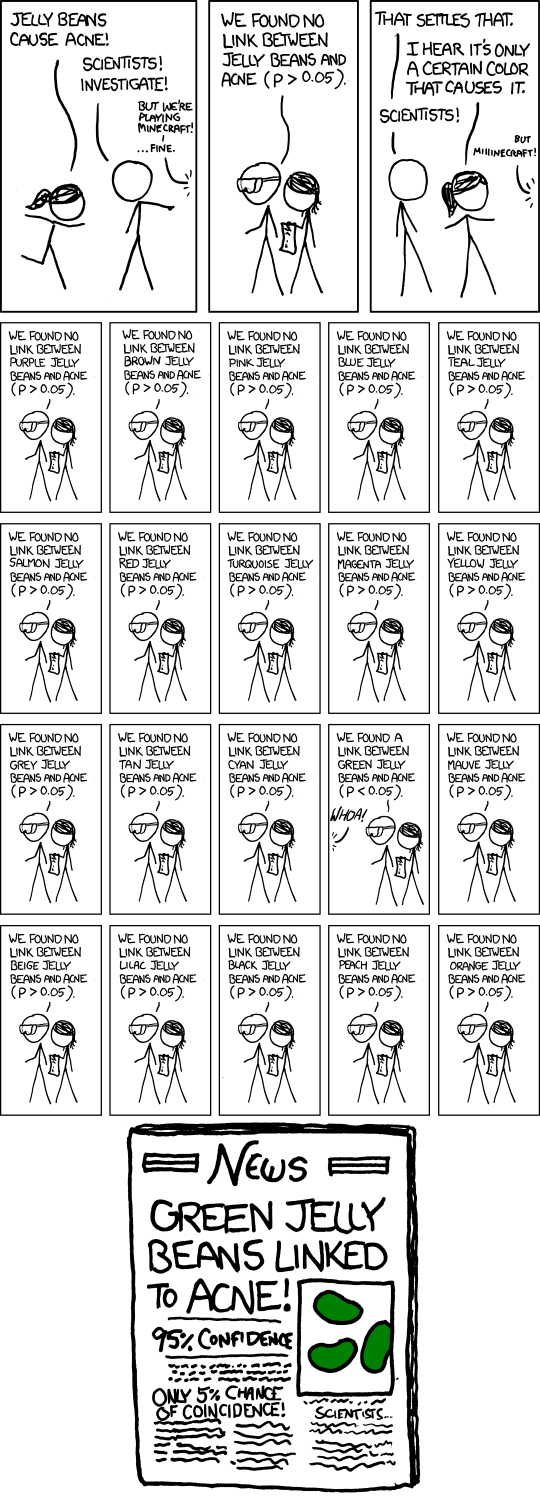
\includegraphics{significant} \end{center}

\hypertarget{false-negatives}{%
\paragraph{False negatives}\label{false-negatives}}

On the other hand, we may also fail to reject the null hypothesis when
the null hypothesis is in fact false. We might just not have enough data
to reject the null, for example. We call this a \emph{false negative} or
a Type II error. We write this as

\[\text{Power} = P(\text{fail to reject} \; H_0 | H_0 \; \text{false}) = 1 - \beta\]

To achieve a power of \(1 - \b\) for a one sample Z-test, you need

\[n \approx \left({\sigma \cdot (z_{\a / 2} + z_\b) \over \mu_0 - \mu_A}\right)^2\]

where \(\mu_A\) is the true mean and \(\mu_0\) is the proposed mean.
We'll do an exercise later that will help you see where this comes from.

\hypertarget{sampling-distributions}{%
\subsubsection{Sampling distributions}\label{sampling-distributions}}

Suppose that \(X_i\) are independent and identically
\(\NormalD{\mu}{\sigma^2}\).

\renewcommand{\arraystretch}{2}

\begin{figure}[h]
  \begin{center}
    \begin{tabular}{lllll}
     known parameters & null hypothesis & test statistic & null distribution \\
     \hline
     $\mu$ unknown, $\sigma^2$ known & $H_0: \mu = \mu_0$ & $\displaystyle {\bar x - \mu_0 \over {\sigma \over \sqrt n}}$ & N(0, 1) \\
     $\mu, \sigma^2$ unknown & $H_0: \mu = \mu_0$ & $\displaystyle {\bar x - \mu_0 \over {s \over \sqrt n}}$ & $t_{n-1}$
    \end{tabular}
  \end{center}
\end{figure}

\hypertarget{examples}{%
\subsection{Examples}\label{examples}}

\hypertarget{z-test}{%
\subsubsection{Z-test}\label{z-test}}

A company claims battery lifetimes are normally distributed with
\(\mu = 40\) and \(\sigma = 5\) hours. We are curious if the claim about
the mean is reasonable, and collect a random sample of 100 batteries.
The sample mean is 39.8. What is the p-value of a Z-test for
\(H_0 : \mu = 40\)?

We begin by calculating a Z-score

\[Z = {\bar x - \mu_0 \over {\sigma \over \sqrt n}} = {39.8 - 40 \over {5 \over \sqrt 100}} = 0.4\]

and then we calulate, using the fact that \(Z \dist \NormalD{0}{1}\),

\[P(Z < -0.4) + P(Z > 0.4) \approx 0.69\]

we might also be interested in a \emph{one-sided} test, where
\(H_A : \mu < 40\). In this case the p-value is only the case when
\(Z < -0.4\), and the p-value is

\[P(Z < -0.4) \approx 0.34\]

\hypertarget{power-for-z-test}{%
\subsubsection{Power for Z-test}\label{power-for-z-test}}

Suppose a powdered medicine is supposed to have a mean particle diameter
of \(\mu = 15\) micrometers, and the standard deviation of diameters
stays steady around 1.8 micrometers. The company would like to have high
power to detect mean thicknesses 0.2 micrometers away from 15. When
\(n = 100\), what is the power of the test if the true \(\mu\) is 15.2
micrometers. Assume the company is interested in controlling type I
error at an \(\a = 0.05\) level.

We will reject the null when our Z score is less than \(z_{\a / 2}\) or
\(z_{1 - \a / 2}\), or when the Z score is less than -1.96 or greater
than 1.96. Recall that the Z score is
\({\bar x - \mu_0 \over {\sigma \over \sqrt n}}\), which we can
rearrange in terms of \(\bar x\) to see that we will reject the null
when \(\bar x < 14.65\) or \(\bar x > 15.35\).

Now we are interested in

\[P(\bar x > 15.35 | \mu = 15.2) + P(\bar x < 14.65 | \mu = 15.2)\]

and we know that \(\bar x \dist \NormalD{15.2}{1.8 / \sqrt{100}}\) so
this equals

\[0.001 + 0.198 \approx 0.199\] So we have only a power of about 20
percent. This is quite low.


\end{document}
